\section{Umsetzung}


\subsection{Laboraufbau}
Um die Simulationen in die Praxis umzusetzen, wurde ein \grqq T-Drive 3Ph compact Thyristorsteller\grqq \hspace{0.03cm} von der Firma Chemtronic, vom Dozenten zur Verfügung gestellt. Wie der Name des Produktes schon sagt, arbeitet dieser Thyristorschaltung mit 3 Phasen. Für die Ansteuerung des Zündwinkels kann ein Potenziometer verwendet werden, dies hat jedoch den Nachteil, dass der Zündwinkel von Hand eingestellt werden muss. Jedoch kann die Ansteuerung auch über ein Spannungssignal von \SI{0}{V} - \SI{10}{V} benutzt werden. Um dieses Spannungssignal erzeugen zu können, wurde ein Arduino Mega 2560 verwendet. Das Problem dabei ist, dass der Arduino nur eine Ausgangsspannung von \SI{5}{V} erzeugen kann. Deshalb wurde eine Spannungsverstärkungsschaltung designt, welche die Spannung verdoppelt. Um die variable Spannung zu erzeugen, wurde im Arduino die PWM-Funktion genutzt. Diese läuft mit einer Frequenz von \SI{490}{Hz}. Für die Ansteuerung sollte aber eine reine DC-Spannung geliefert werden. Deshalb wurde zusätzlich ein Tiefpass-Filter erster Ordnung am Ausgang des Arduinos eingebaut, mit einer Cut-off Frequenz von \SI{1}{Hz}.  


\subsubsection{Filter}
Um die Elemente des Tiefpassfilters zu berechnen, wurde folgende Formel verwendet.
\begin{equation}
f = \frac{1}{2 \cdot \pi \cdot R_1 \cdot C_1}
\end{equation}
Dabei wurde $f$ = \SI{1}{Hz} eingesetzt und so kann die Kapazität oder der Widerstand frei gewählt werden. Für die Kapazität wurde \SI{10}{\mu F} ausgesucht. Somit ergab sich einen Widerstand von \SI{16}{\Omega}. 


\subsubsection{Verstärkerschaltung}
Die Verstärkung einer nicht invertierenden Verstärkungsschaltung wird wie folgt berechnet.
\begin{equation}
V_u = 1 + \frac{R_3}{R_2}
\end{equation}
Um die Ströme klein zu halten, wurden Widerstände von \SI{12}{k\Omega} ausgewählt. Um eine Verstärkung von zwei zu erreichen, wurden die beiden Widerstände gleich gross gewählt. 

Diese Schaltung wurde zusätzlich noch im Plecs simuliert.

\todo{evt. einfügen grafik Plecs}


\begin{figure}[ht!]  
	\centering 
	\begin{minipage}[t]{.76\textwidth} \centering 
		\centering
		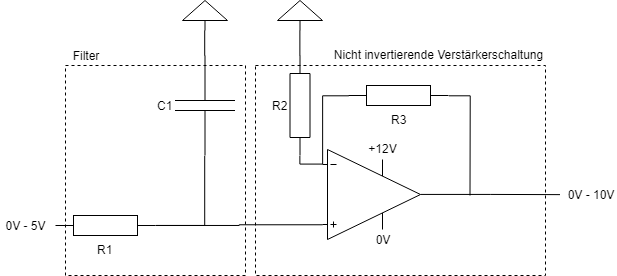
\includegraphics[scale=0.555]{Schema_Verstaerkerschaltung.png}	
		\caption{Schema Verstärkerschaltung}\label{fig:Verstaerkerschaltung}
	\end{minipage}	
% 
	\begin{minipage}[b]{.23\textwidth}
	\centering
		\begin{tabular}{|l|l|}
			\hline
			R$_1$ & \SI{16}{k\Omega} 	\\ 	\hline
			R$_2$ & \SI{12}{k\Omega} 	\\ 	\hline
			R$_3$ & \SI{12}{k\Omega} 	\\	\hline
			C$_1$ & \SI{10}{\mu F} 		\\	\hline
		\end{tabular}
		\caption{Werte der Bauteile}
		\label{tab:Verstaerkerschaltung}
	\end{minipage}
\end{figure} 



Nach dem Aufbau der Verstärkerschaltung wurde die Ausgangsspannung bei einem duty-cycle von 1 gemessen. Dabei wurde ein Wert von \SI{9.885}{V} gemessen. Dies bedeutet das der Thyristorsteller nicht voll ausgesteuert werden kann. Deshalb wurde bei der Verstärkerschaltung die Verstärkung erhöht. 

\begin{equation}
\frac{12k\Omega}{11k\Omega} = 1.09
\end{equation}
Dies resultiert in eine Verstärkung von:
\begin{equation}
V_u = 1 + \frac{12k\Omega}{11k\Omega} = 2.09
\end{equation}
Nach dem Einbau des neuen Widerstandes wurde eine Spannung von \SI{10.2}{V} am Ausgang gemessen. Somit kann der Thyristorsteller voll ausgesteuert werden.

\subsection{Laboraufbau mit Widerstand}
Nach dem Feststellen der Funktionalität der Spannnungsverstärkungsschaltung konnte mit dem Laboraufbau begonnen werden. Hierzu wurde ein variabler Culatti-Widerstand als Last benutzt. Dieser hat den Vorteil das die Last bei allen Phasen symetrisch ist. Um den Strom klein zu halten, wurde ein Widerstand von \SI{150}{\Omega} gewählt. Der Aufbau der Messschaltung ist auf der Abbildung \ref{fig:Messaufbau} ersichtlich. 

\begin{figure}[ht!]
	\centering
	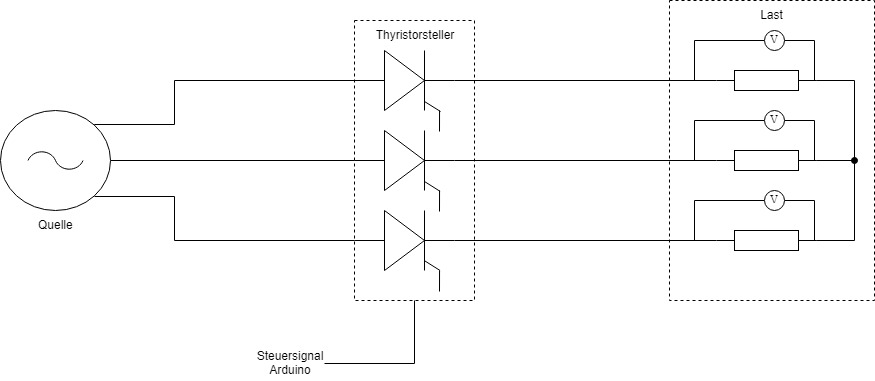
\includegraphics[width=\textwidth]{Messaufbau.png}	
	\caption{Schema Messaufbau}\label{fig:Messaufbau}
\end{figure}

Um zu analysieren wie sich die Spannung bei der Last in Dreieck verläuft, konnte die Last auch in Dreieck geschaltet werden.


\subsection{Arduino}
Das Arduino-Programm, welches den Thyristorsteller ansteuert, wurde mit der Arduinosoftware geschrieben. Dabei werden die Steuerungsspannung mit einem PWM generiert. Dieser fährt mit einer for-Schleife von \SI{0}{V} bis \SI{5}{V} hoch. Danach bleibt der PWM für eine Zeit auf dem Maximum und fährt dann wieder runter. Zusätzlich wurde eine for-Schleife gemacht, welche die Schwingungspaketsteuerung macht. Dazu werden eine gewisse Anzahl vom PWM eingeschaltet und andere werden gesperrt. \todo{Code in Anhang}


\subsubsection{Schwingungspaketsteuerung mit Arduino}



\subsubsection{Phasenanschnittssteuerung mit Arduino}

\newpage
\subsection{Messungen}

\subsubsection{Schwingungspaketsteuerung mit Last in Stern}
Für die Messung mit der Schwingungspaketsteuerung wurde eine Einschaltzeit von 0.5 Sekunden und eine Ausschaltzeit von 0.2 Sekunden gewählt. Die Ausschaltzeit darf nicht kürzer sein, da die Spannungsverstärkerschaltung und den Thyristorsteller eine Zeitverzögerung darstellen und so die Spannung nicht sofort ein- oder ausgeschaltet wird. Wenn die Ausschaltzeit kürzer ist, geht die Spannung zwischen den Paketen nicht auf \SI{0}{V}. 
\begin{figure}[ht!]
	\centering
	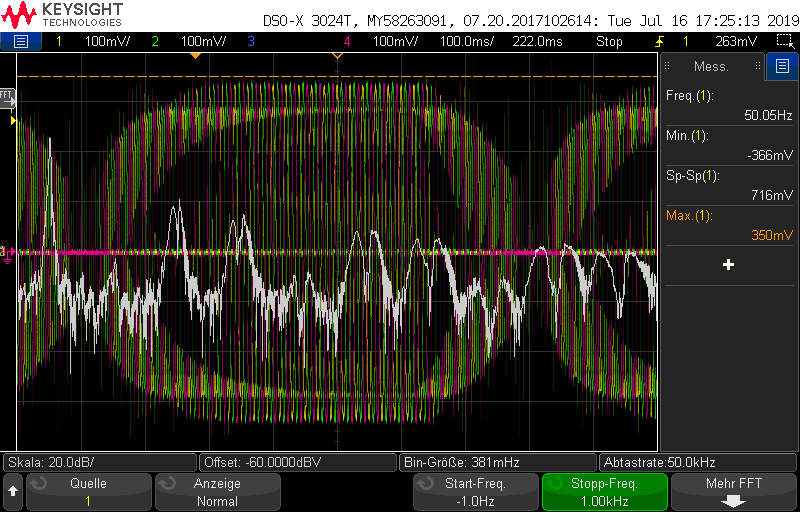
\includegraphics[width=0.7\textwidth]{Schwingungspaket_kurz.png}	
	\caption{Das Spannungssignal aller Phasen bei Schwingungspaketsteuerung mit FFT}\label{fig:Mess_Schwing_kurz}
\end{figure}

Das FFT zeigt entgegen den Erwartungen aus der Theorie fast keine Subharmonische auf. Dafür sind Harmonische und Zwischehamrnische sehr ausgeprägt. Sehr gut zu sehen ist die Grundfrequenz von \SI{50}{Hz}, der erste Peak von der linken Seite. Dies ist darauf zurückzuführen, dass nicht direkt ein- und ausgeschaltet wird und so einem Sanft-Anlass ähnelt. Dies dominiert gegenüber dem harten Ein- und Ausschalten, welches die Subharmonische hervorrufen würde.
\newpage
\subsection{Phasenanschnittsteuerung mit 2 Thyristoren mit Last in Stern}
Für die Sparansteuerung wurde ein Winkel von 90\textdegree gewählt. 

\begin{figure}[ht!]
	\centering
	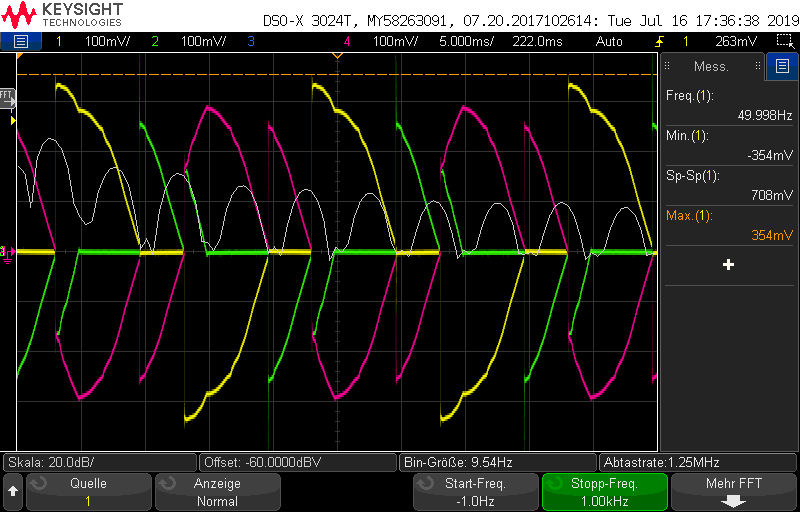
\includegraphics[width=0.7\textwidth]{2phas_90grad_kurz.png}	
	\caption{Das Spannungssignal aller Phasen bei Schwingungspaketsteuerung mit FFT}\label{fig:Mess_2phas_kurz}
\end{figure}


\subsection{Phasenanschnittsteuerung mit 1 Thyristor mit Last in Stern}
Für die Sparansteuerung wurde ein Winkel von 90\textdegree gewählt. 

\begin{figure}[ht!]
	\centering
	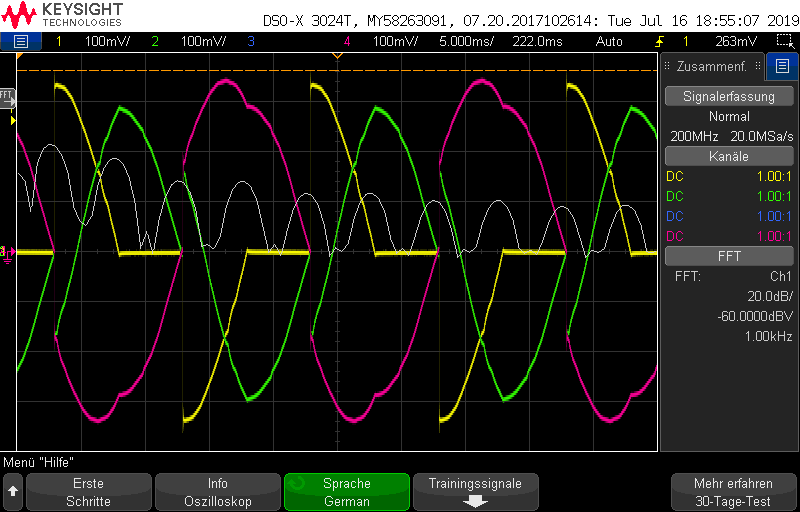
\includegraphics[width=0.7\textwidth]{1phas_90grad_kurz.png}	
	\caption{Das Spannungssignal aller Phasen bei Schwingungspaketsteuerung mit FFT}\label{fig:Mess_1phas_kurz}
\end{figure}





